

The components of the velocity are obtained from the stream function as follows:
\[
u = \frac{1}{r}\frac{\partial \Psi}{\partial \theta}
\quad\quad
v = - \frac{\partial \Psi}{\partial r}
\]
where $u$ is the radial component and $v$ is the tangential component.
In polar coordinates the curl of a vector ${\bm A}$ is:
\[
{\bm \nabla}\times {\bm A}
=
\frac{1}{r}\left(  
\frac{\partial (r A_\theta)}{\partial r}
-
\frac{\partial A_r}{\partial \theta}
\right)
\]
and the Laplacian of any scalar function $f$ is 
\[
\Delta f = \frac{1}{r} \frac{\partial }{\partial r} \left( r  \frac{\partial f}{\partial r} \right) 
+  \frac{1}{r^2} \frac{\partial^2 f}{\partial \theta^2} 
\]
The Stokes equations are
\begin{eqnarray}
A_r=-\frac{\partial p}{\partial r} + \eta \Delta u &=& \rho g_r \\
A_\theta=-\frac{1}{r}\frac{\partial p}{\partial \theta} + \eta \Delta v &=& \rho g_\theta 
\end{eqnarray}
Taking the curl of vector ${\bm A}$ yields:
\[
\frac{1}{r}\left(  
\frac{\partial (r A_\theta)}{\partial r}
- \frac{\partial A_r}{\partial \theta}
\right)
=
\frac{1}{r}\left(  
\frac{\partial (r \rho g_\theta)}{\partial r}
- \frac{\partial (\rho g_r)}{\partial \theta}
\right)
\]
Multiplying on each side by $r$ and assuming the gravity vector is radial ($g_\theta=0$):
\[
\frac{\partial (r A_\theta)}{\partial r}
- \frac{\partial A_r}{\partial \theta}
=
- \frac{\partial \rho g_r}{\partial \theta}
\]
If we now replace $A_r$ and $A_\theta$ by their expressions as a function of velocity and pressure, 
we see that the pressure terms cancel out so that only the Laplacian terms remain:
\[
\frac{\partial (r \eta \Delta v)}{\partial r}
- \frac{\partial (\eta \Delta u)}{\partial \theta}
=
- \frac{\partial \rho g_r}{\partial \theta}
\]
Assuming the viscosity and the gravity vector to be constant:
\[
\frac{\partial (r  \Delta v)}{\partial r}
- \frac{\partial  \Delta u}{\partial \theta}
=
- \frac{1}{\eta} \frac{\partial \rho }{\partial \theta} g_r
\]
Then
\begin{eqnarray}
\frac{\partial (r  \Delta v)}{\partial r}
&=&
\frac{\partial}{\partial r} \left(   \frac{\partial }{\partial r} \left( r  \frac{\partial v}{\partial r} \right) +  \frac{1}{r} \frac{\partial^2 v}{\partial \theta^2}  \right) \\
&=&
\frac{\partial^2 }{\partial r^2} \left( r  \frac{\partial v}{\partial r} \right) 
+ \frac{\partial }{\partial r} \left( \frac{1}{r} \frac{\partial^2 v}{\partial \theta^2} \right) \\
&=&
\frac{\partial^2 }{\partial r^2} \left( r  \frac{\partial }{\partial r} ( - \frac{\partial \Psi}{\partial r}  ) \right) + \frac{\partial }{\partial r} \left( \frac{1}{r} \frac{\partial^2 }{\partial \theta^2} (- \frac{\partial \Psi}{\partial r}) \right) \\ 
&=&
- \frac{\partial^2 }{\partial r^2} \left( r    \frac{\partial^2 \Psi}{\partial r^2}   \right) - \frac{\partial }{\partial r} \left( \frac{1}{r} \frac{\partial^3 \Psi}{\partial \theta^2 \partial r}  \right) \\ 
&=& - 2  \frac{\partial^3 \Psi}{\partial r^3}  -  r \frac{\partial^4 \Psi}{\partial r^4}
+\frac{1}{r^2} \frac{\partial^3 \Psi}{\partial \theta^2 \partial r}  
- \frac{1}{r} \frac{\partial^4 \Psi}{\partial \theta^2 \partial r^2}
\\
\frac{\partial  \Delta u}{\partial \theta}
&=& \frac{\partial }{\partial \theta} \left(
\frac{1}{r} \frac{\partial }{\partial r} \left( r  \frac{\partial u}{\partial r} \right) 
+  \frac{1}{r^2} \frac{\partial^2 u}{\partial \theta^2}  \right)\\
&=& \frac{\partial }{\partial \theta} \left(
\frac{1}{r} \frac{\partial }{\partial r} \left( r  \frac{\partial u}{\partial r} \right) \right)
+  \frac{1}{r^2} \frac{\partial^3 u}{\partial \theta^3}  \\
&=& \frac{\partial }{\partial \theta} \left(
\frac{1}{r} \frac{\partial }{\partial r} \left( r  \frac{\partial }{\partial r} (  \frac{1}{r}\frac{\partial \Psi}{\partial \theta}  ) \right) \right)
+  \frac{1}{r^2} \frac{\partial^3 }{\partial \theta^3}( \frac{1}{r}\frac{\partial \Psi}{\partial \theta})  \\
&=&
\frac{1}{r^3} \frac{\partial^2 \Psi}{\partial \theta^2} - 
\frac{1}{r^2} \frac{\partial^3 \Psi}{\partial r \partial \theta^2} +
\frac{1}{r} \frac{\partial^4 \Psi}{\partial r^2 \partial \theta^2} +
\frac{1}{r^3} \frac{\partial^4 \Psi}{\partial \theta^4} 
\end{eqnarray}

Assuming the following separation of variables $\boxed{\Psi(r,\theta)=\phi(r)\xi(\theta)}$:
\begin{eqnarray}
\frac{\partial (r  \Delta v)}{\partial r}
&=& -2 \phi''' \xi - r \phi'''' \xi + \frac{1}{r^2} \phi' \xi''  - \frac{1}{r} \phi'' \xi'' \\
\frac{\partial  \Delta u}{\partial \theta}
&=&
\frac{1}{r^3} \phi \xi '' -
\frac{1}{r^2} \phi' \xi'' +
\frac{1}{r} \phi'' \xi'' +
\frac{1}{r^3} \phi \xi''''
\end{eqnarray}
so that 
\[
\frac{\partial (r  \Delta v)}{\partial r} - \frac{\partial  \Delta u}{\partial \theta}
=  -2 \phi''' \xi - r \phi'''' \xi + \frac{1}{r^2} \phi' \xi''  - \frac{1}{r} \phi'' \xi'' 
-\frac{1}{r^3} \phi \xi '' +
\frac{1}{r^2} \phi' \xi'' -
\frac{1}{r} \phi'' \xi'' -
\frac{1}{r^3} \phi \xi''''
\]
Further assuming $\boxed{\xi(\theta)=\cos(k\theta)}$, then $\xi''=-k^2 \xi$ and $\xi''''=k^4 \xi$
then 
\[
\frac{\partial (r  \Delta v)}{\partial r} - \frac{\partial  \Delta u}{\partial \theta}
=  -2 \phi''' \xi - r \phi'''' \xi - k^2 \frac{1}{r^2} \phi' \xi  +k^2 \frac{1}{r} \phi'' \xi 
+ k^2\frac{1}{r^3} \phi \xi  
-k^2\frac{1}{r^2} \phi' \xi 
+k^2 \frac{1}{r} \phi'' \xi 
- k^4\frac{1}{r^3} \phi \xi
\]
By choosing $\rho$ such that $\rho= f(r)g(\theta)$ and such that $\partial_\theta g = \xi$
then we have 
\[
 -2 \phi''' \xi - r \phi'''' \xi - k^2 \frac{1}{r^2} \phi' \xi  +k^2 \frac{1}{r} \phi'' \xi 
+ k^2\frac{1}{r^3} \phi \xi  
-k^2\frac{1}{r^2} \phi' \xi 
+k^2 \frac{1}{r} \phi'' \xi 
- k^4\frac{1}{r^3} \phi \xi
=
- \frac{1}{\eta} f \xi  g_r
\]
and then dividing by $\xi$: (IS THIS OK ?)
\[
 -2 \phi'''  - r \phi''''  - k^2 \frac{1}{r^2} \phi'   +k^2 \frac{1}{r} \phi''  
+ k^2\frac{1}{r^3} \phi 
-k^2\frac{1}{r^2} \phi' 
+k^2 \frac{1}{r} \phi'' 
- k^4\frac{1}{r^3} \phi 
=
- \frac{1}{\eta} f   g_r
\]

\[
-2 \phi'''  - r \phi''''  
- 2k^2 \frac{1}{r^2} \phi'   
+2k^2 \frac{1}{r} \phi''  
+ (k^2-k^4) \frac{1}{r^3} \phi 
=
- \frac{1}{\eta} f   g_r
\]
so 


\[
\boxed{
f(r) = \frac{\eta}{g} \left( 
2 \phi'''  + r \phi''''  + 2k^2 \frac{1}{r^2} \phi'   
-2k^2 \frac{1}{r} \phi''  
- (k^2-k^4) \frac{1}{r^3} \phi 
\right)
}
\]

%%%%%%%%%%%%%%%%%%%%%%%%%%%%%%%%%%%%%%%%%%%%%%%%%%5
\subsection{No slip boundary conditions}

No-slip boundary conditions inside and outside impose that all components of the velocity
must be zero on both boundaries, i.e.
\[
{\bm v}(r=R_1)={\bm v}(r=R_2)={\bm 0}
\]
Due to the separation of variables, and since  $\xi(\theta)=\cos(k\theta)$ we have
\[
u(r,\theta) = \frac{1}{r}\frac{\partial \Psi}{\partial \theta} 
=\frac{1}{r} \phi \xi' 
=-\frac{1}{r} \phi(r) k \sin(k \theta) 
\quad\quad\quad
v(r,\theta) = - \frac{\partial \Psi}{\partial r} 
= - \phi'(r) \xi 
= - \phi'(r) \cos(k\theta)
\]
It is obvious that the only way to insure no-slip boundary conditions is to have 
\[
\phi(R_1)=\phi(R_2)=\phi'(R_1)=\phi'(R_2)=0
\]
We could then choose
\begin{eqnarray}
\phi(r)&=&(r-R_1)^2(r-R_2)^2 {\cal F}(r) \\
\phi'(r)&=&2(r-R_1)(r-R_2)^2 {\cal F}(r)  +2(r-R_1)^2(r-R_2) {\cal F}(r) +(r-R_1)^2(r-R_2)^2 {\cal F}'(r)
\end{eqnarray}
which are indeed identically zero on both boundaries. Here ${\cal F}(r)$ is any (smooth enough) function of $r$.
We would then have
\[
\boxed{
\Psi(r,\theta) = (r-R_1)^2(r-R_2)^2 {\cal F}(r) \cos(k\theta)
}
\]
In what follows we will take ${\cal F}(r)=1$ for simplicity.

\begin{center}
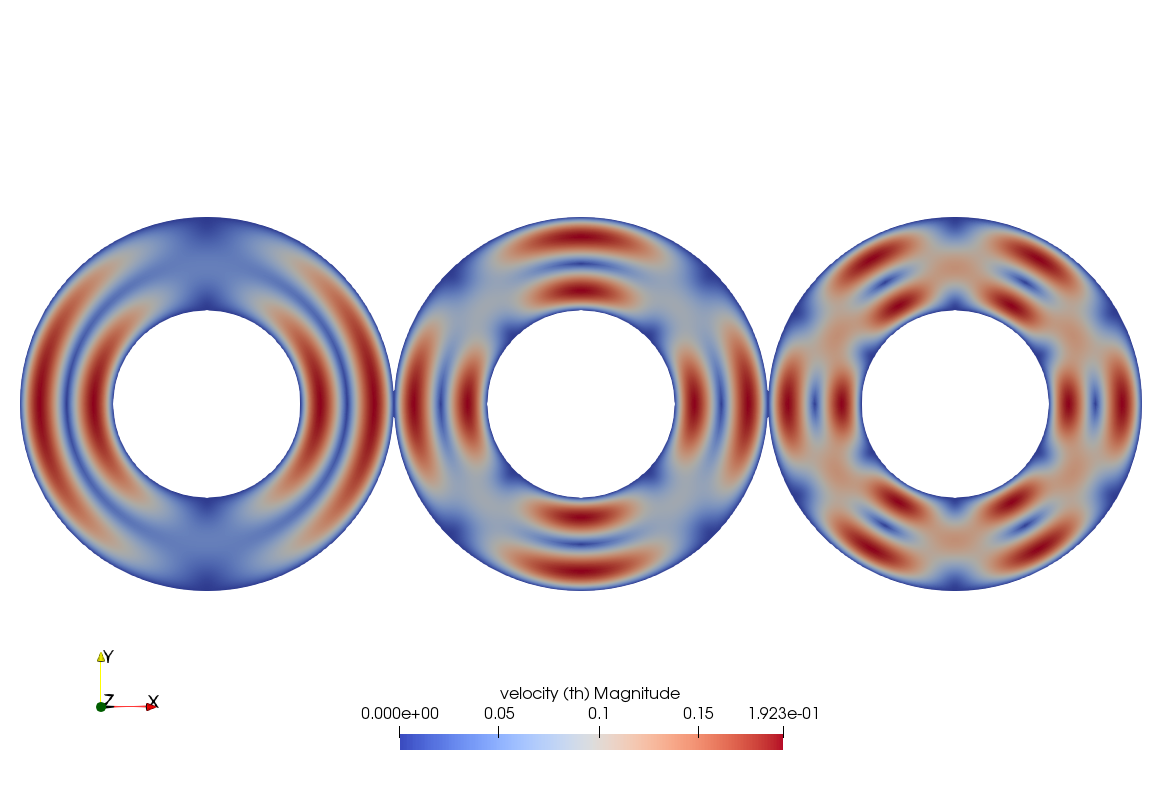
\includegraphics[width=12cm]{python_codes/fieldstone_35/images/vels}
\end{center}

COMPUTE $f$ from $\phi$ and then the pressure.


%%%%%%%%%%%%%%%%%%%%%%%%%%%%%%%%%%%%%%%%%%%%%%%%%%5
\subsection{Free slip boundary conditions}

Before postulating the form of $\phi(r)$, let us now turn to the boundary conditions that the flow must fulfill, i.e. free-slip on both boundaries.
Two conditions must be met:

\begin{itemize}
\item ${\bm v} \cdot {\bm n}=0$ (no flow through the boundaries) which yields $u(r=R_1)=0$ and $u(r=R_2)=0$, :
\[
\frac{1}{r}\frac{\partial \Psi}{\partial \theta} (r=R_1,R_2)=0   \quad\quad \forall \theta
\]
which gives us the first constraint since $\Psi(r,\theta)=\phi(r)\xi(\theta)$:
\[
\phi(r=R_1)=\phi(r=R_2)=0  
\]
\item $({\bm \sigma} \cdot {\bm n}) \times {\bm n} = {\bm 0} $  (the tangential stress at the boundary is zero)
which imposes: $\sigma_{\theta r}=0$, with
\[
\sigma_{\theta r}=
2 \eta \cdot \frac{1}{2} \left( \frac{\partial v}{\partial r} - \frac{v}{r} + \frac{1}{r} \frac{\partial u}{\partial \theta}    \right)
= \eta \left( \frac{\partial }{\partial r} (- \frac{\partial \Psi}{\partial r}) -
\frac{1}{r} (- \frac{\partial \Psi}{\partial r}) + \frac{1}{r} \frac{\partial }{\partial \theta} (\frac{1}{r}\frac{\partial \Psi}{\partial \theta})    \right)
\]
Finally $\Psi$ must fulfill (on the boundaries!):
\[
-\frac{\partial^2 \Psi}{\partial r^2} + \frac{1}{r}  \frac{\partial \Psi}{\partial r} + \frac{1}{r^2} \frac{\partial^2 \Psi}{\partial \theta^2}=0
\]
or, 
\[
- \phi'' \xi + \frac{1}{r} \phi' \xi +  \frac{1}{r^2}  \phi \xi'' = 0
\]
\newpage
%Since $\xi''=-k^2 \xi$ and 
Since we are looking for a solution $\phi$ such that $\phi(r=R_1)=\phi(r=R_2)=0 $ then we have to ensure the following equality on the boundary:
\[
- \phi'' \xi + \frac{1}{r} \phi' \xi  = 0
\]
or,
\[
- r \phi''  + \phi' = 0  \quad\quad \text{for} \quad r=R_1,R_2
\]

I then postulate $\phi(r)=(r-R_1)(r-R_2)\chi(r)$ so that it automatically fulfills $\phi(r=R_1)=\phi(r=R_2)=0 $. 
We then have
\begin{eqnarray}
\phi(r) &=& (r-R_1)(r-R_2)\chi(r) \\
\phi'(r) &=& [2r-(R_1+R_2)] \chi(r) + (r-R_1)(r-R_2)\chi'(r) \\
\phi''(r) &=& 2\chi(r) +   2[2r-(R_1+R_2)] \chi'(r) + (r-R_1)(r-R_2)\chi''(r)\\
-r\phi''(r) &=& - 2r\chi(r) -   2r[2r-(R_1+R_2)] \chi'(r) - r(r-R_1)(r-R_2)\chi''(r)
\end{eqnarray}
\[
 - 2r\chi(r) -   2r[2r-(R_1+R_2)] \chi'(r) - r(r-R_1)(r-R_2)\chi''(r) 
+[2r-(R_1+R_2)] \chi(r) + (r-R_1)(r-R_2)\chi'(r) =0
\]
\[
-   2r[2r-(R_1+R_2)] \chi'(r) 
-(R_1+R_2) \chi(r) 
- r(r-R_1)(r-R_2)\chi''(r) 
+ (r-R_1)(r-R_2)\chi'(r) =0
\]


Then the function $\chi$ must fulfill:
\begin{eqnarray}
0 =-R_1\phi''(R_1) + \phi'(R_1) 
&=& - 2R_1\chi(R_1) -  2R_1[R_1-R_2] \chi'(R_1) +[R_1-R_2] \chi(R_1)  \\
&=& -  2R_1[R_1-R_2] \chi'(R_1) - [R_1+ R_2] \chi(R_1)  \\
0=-R_2\phi''(R_2) + \phi'(R_2) 
&=& - 2R_2\chi(R_2) + 2R_2[R_1-R_2] \chi'(R_2) -[R_1-R_2] \chi(R_2) \\
&=&  2R_2[R_1-R_2] \chi'(R_2) -[R_1+R_2] \chi(R_2) 
\end{eqnarray}

http://mathworld.wolfram.com/EulerDifferentialEquation.html


\end{itemize}

{\color{red} I am stuck here}








